\documentclass[dvipdfmx]{beamer}

\usepackage{graphicx,color}

%読めない、意味分からないのでコメントアウト。なくても動くし
%\usepackage{siunitx}

\usepackage{comment}
\usepackage{listings, jlisting}
\usepackage{fancyvrb}
\usepackage{subfigure}
\usepackage[font=footnotesize]{caption}

% 図表番号を振る
\setbeamertemplate{caption}[numbered]

% 下の図表番号のスペースを除去
\setlength\abovecaptionskip{0.5em}

\newenvironment{wideitemize}{\itemize\setlength{\itemsep}{1em}}{\enditemize}
\newenvironment{wideitemize2}{\itemize\setlength{\itemsep}{0.2em}}{\enditemize}
\newenvironment{widedescription}{\description\setlength{\itemsep}{1em}}{\enddescription}
\newenvironment{widedescription2}{\description\setlength{\itemsep}{0.2em}}{\enddescription}

\lstset{language=C++,
    basicstyle=\ttfamily\scriptsize,
    keywordstyle=\color{blue}\ttfamily,
    stringstyle=\color[cmyk]{0,0.6,1,0.2}\ttfamily,
    commentstyle=\color[cmyk]{1,0.4,1,0}\ttfamily,
    identifierstyle=\color[cmyk]{0,1,0.1,0.8}\ttfamily,
    morecomment=[l][\color{magenta}]{\#},
    breaklines = true
}

%\usetheme{Rochester}
\usetheme{Madrid}
\usecolortheme{seahorse}

\title[2015年度初年次ゼミ問題]{具体的な問題}
\subtitle{}
\author[遠藤 亘 岩崎 慎太郎]{遠藤 亘 岩崎 慎太郎}
\institute[田浦研]{情報理工学系研究科 修士1年 田浦研究室}
\date{2015-06-12}

\begin{document}

\begin{frame}
\titlepage
\end{frame}


%%%%%%%%%%%%%%%%%%%%%%%%%%%%%%%%%%%%%%%%%%%%%%%%%%%%%%%%%%%%%%%%%%%%%%%%%%%%%%%%%%%%%%%%%%%%%%%%%%%%%%%%%%%%

\begin{frame}{問題1}{熱伝導}
\begin{columns}[t]
\begin{column}{0.7\textwidth}
\begin{wideitemize}
	\item 側面が断熱された温度$T_0$、長さ$L$、の細い銅の棒がある。
	両端をそれぞれ$T_1$、$T_2$の温度で維持する時、金属棒の温度の変化を求めよ。
	\begin{wideitemize2}
		\item 他の金属(鉄、アルミニウム、銀)などでも試し、時間変化や結果を比較せよ。
	\end{wideitemize2}

\end{wideitemize}

\end{column}
\begin{column}{0.3\textwidth}
\begin{figure}[htbp]
    \centering
    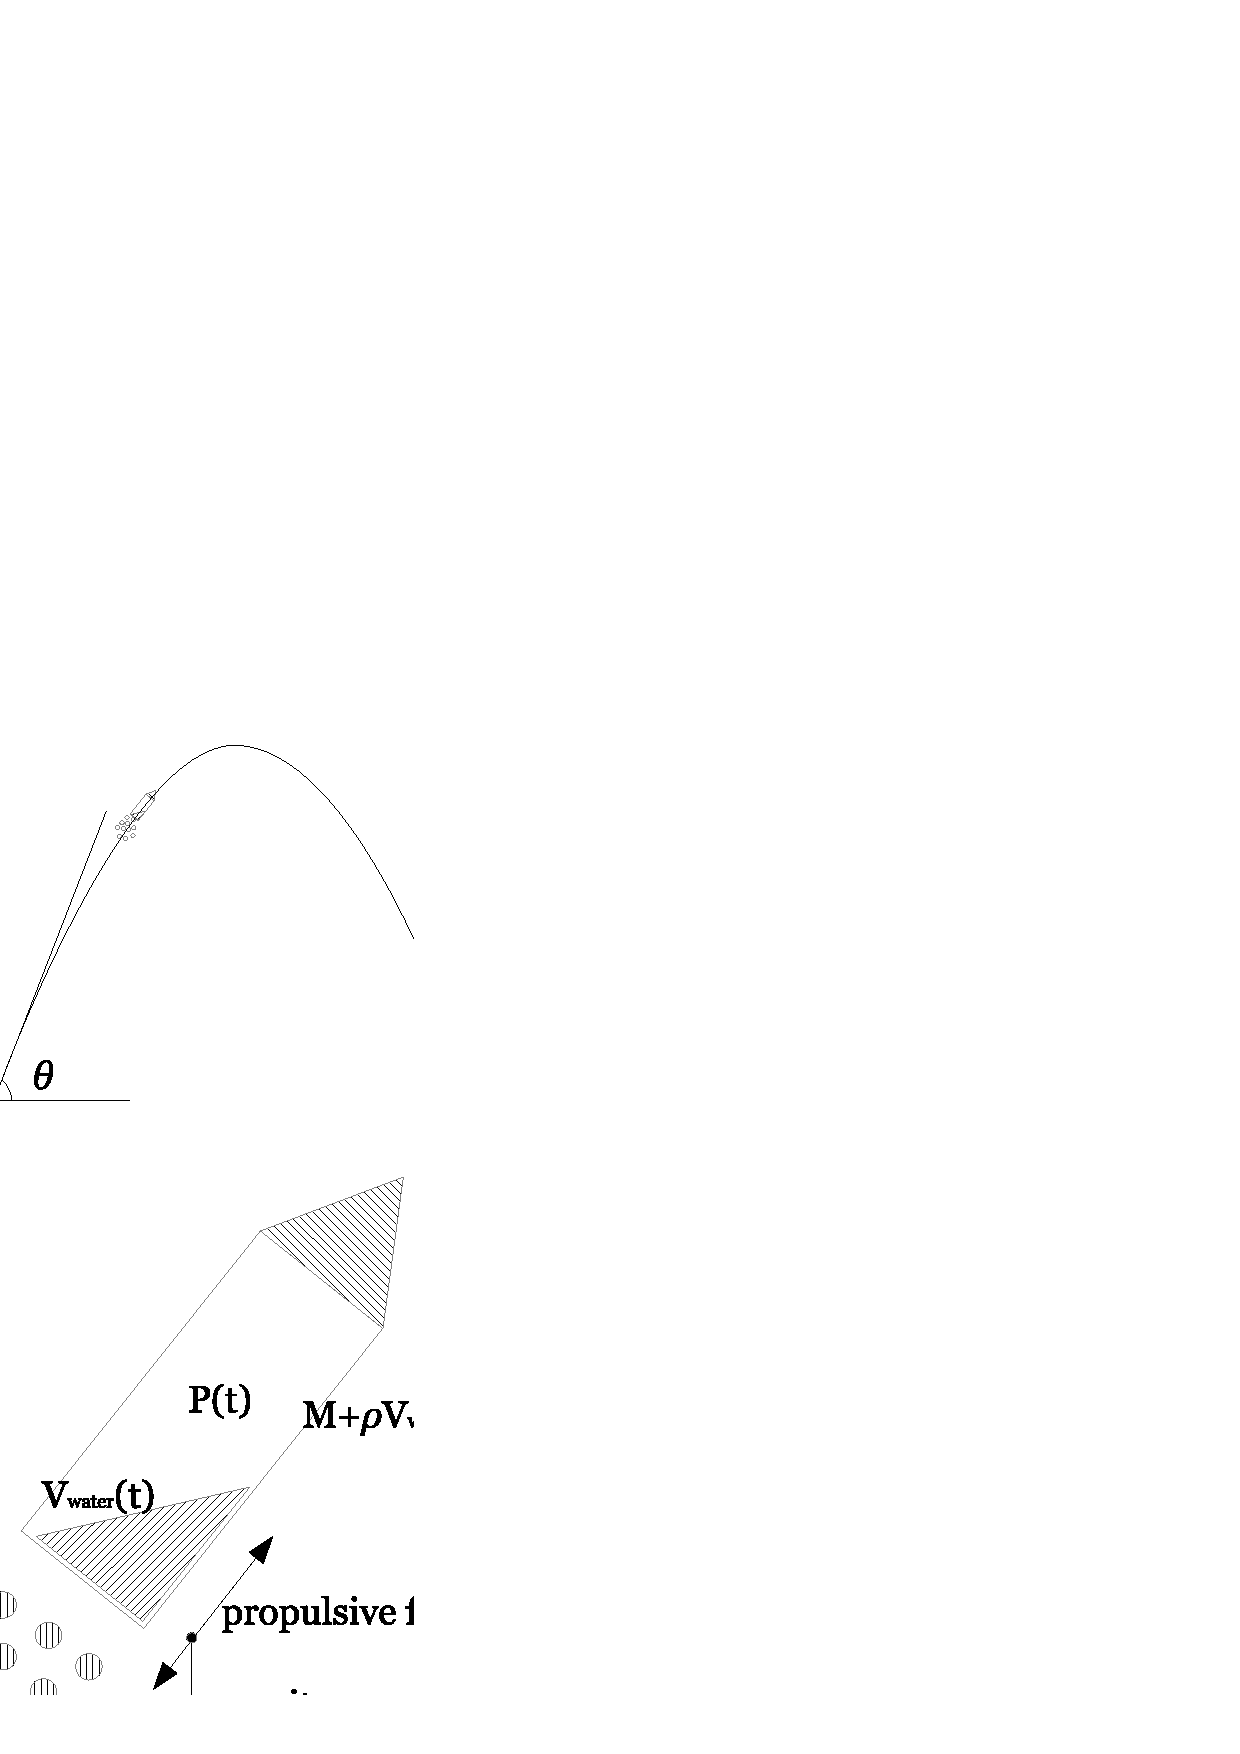
\includegraphics[bb=0mm 0mm 100.0mm 170.0mm, scale=0.35, type=pdf]{img/problem1.pdf}
\end{figure}
\end{column}
\end{columns}
\end{frame}


%%%%%%%%%%%%%%%%%%%%%%%%%%%%%%%%%%%%%%%%%%%%%%%%%%%%%%%%%%%%%%%%%%%%%%%%%%%%%%%%%%%%%%%%%%%%%%%%%%%%%%%%%%%%

\begin{frame}{問題2}{球充填}
\begin{columns}[t]
\begin{column}{0.7\textwidth}
\begin{wideitemize}
	\item 物理シミュレーションを用いて、底面が一辺aの立方体に、半径rの球を詰めることを考える。
	球はいくつ入れることができるだろうか?
	\begin{wideitemize2}
		\item aが大きければ、最密充填可能であると考えられる。
	\end{wideitemize2}

\end{wideitemize}

\end{column}
\begin{column}{0.3\textwidth}
\begin{figure}[htbp]
    \centering
    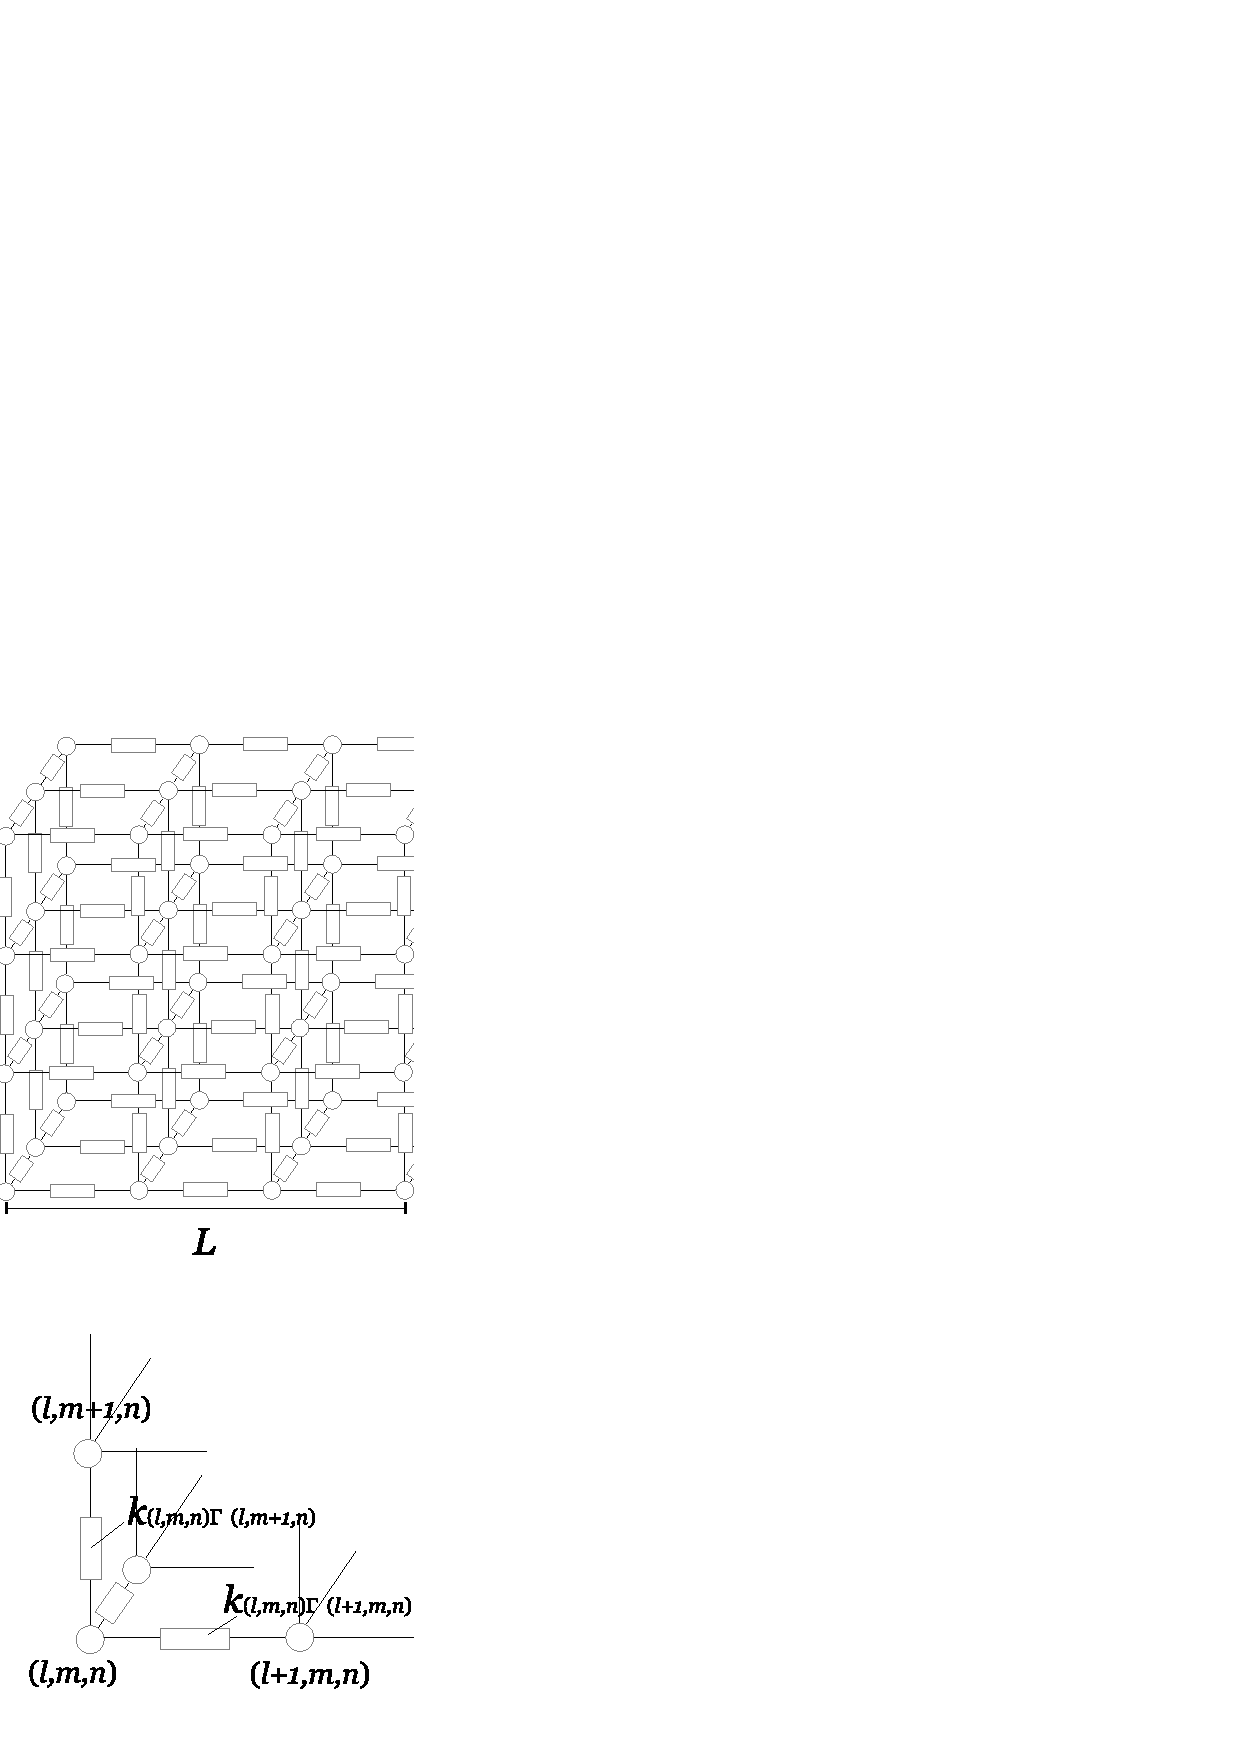
\includegraphics[bb=0mm 0mm 100.0mm 170.0mm, scale=0.35, type=pdf]{img/problem2.pdf}
\end{figure}
\end{column}
\end{columns}
\end{frame}


%%%%%%%%%%%%%%%%%%%%%%%%%%%%%%%%%%%%%%%%%%%%%%%%%%%%%%%%%%%%%%%%%%%%%%%%%%%%%%%%%%%%%%%%%%%%%%%%%%%%%%%%%%%%

\begin{frame}{問題3}{探査衛星とスイングバイ}
\begin{columns}[t]
\begin{column}{0.7\textwidth}
\begin{wideitemize}
	\item 太陽系外に探査機を打ち出したい。打ち上げ日時と位置を求めよ。
	\begin{wideitemize2}
		\item (ボイジャーの打ち上げられた)1970年代に打ち上げる。
		\item 最初のスイングバイまでに太陽を一周しない。
		\item 地上発射時の初速は14.2km/sで、地球を黄道面で切った時の断面円周上のどこから打ち上げても良い
		\item 探査機の重さは750kg。ロケットからの分離は考えない
		\item 惑星(太陽~土星まで)は太陽を中心に円軌道を描き、全て同一平面上で運動するとする
		\item 地球の自転の影響を無視して地上から垂直に打ち上げたとする
	\end{wideitemize2}
\end{wideitemize}

\end{column}
\begin{column}{0.3\textwidth}
\begin{figure}[htbp]
    \centering
    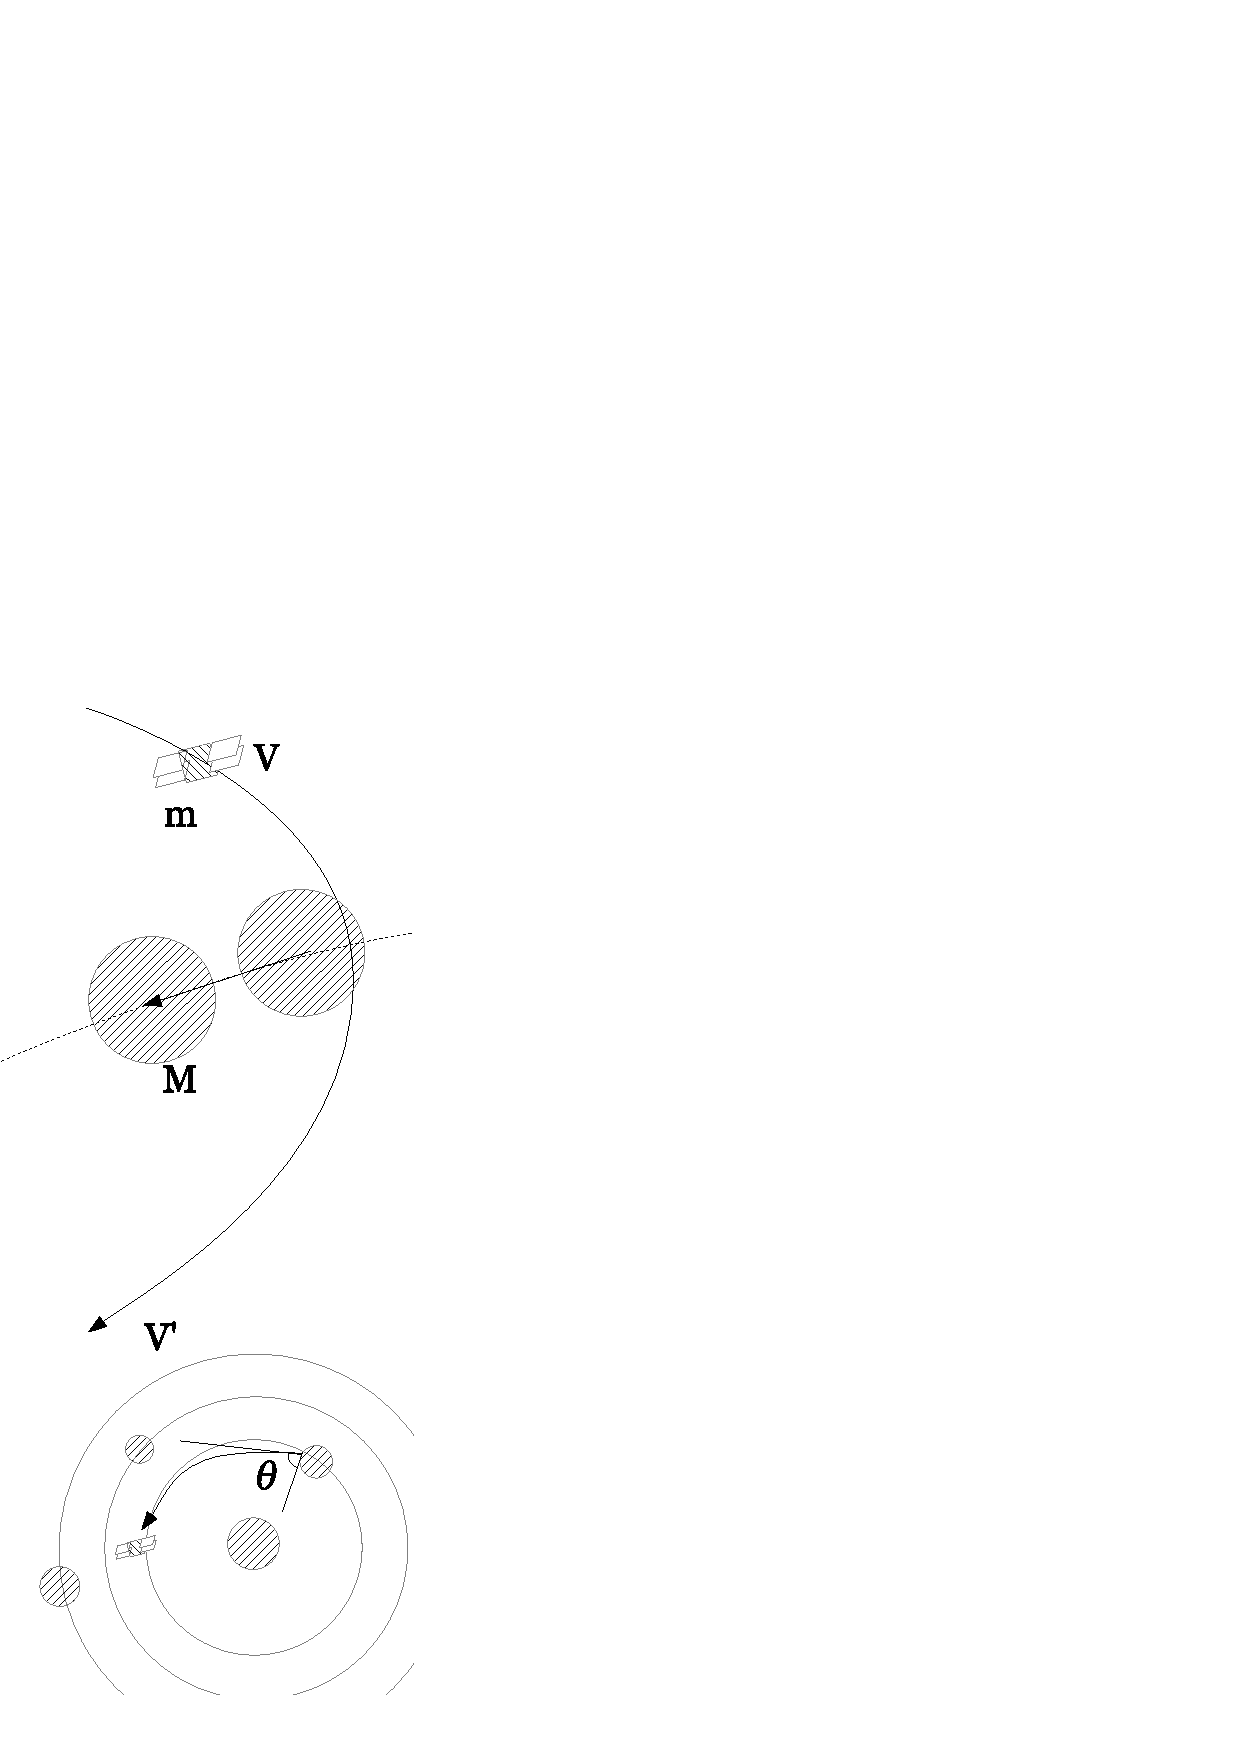
\includegraphics[bb=0mm 0mm 100.0mm 170.0mm, scale=0.35, type=pdf]{img/problem3.pdf}
\end{figure}
\end{column}
\end{columns}
\end{frame}


%%%%%%%%%%%%%%%%%%%%%%%%%%%%%%%%%%%%%%%%%%%%%%%%%%%%%%%%%%%%%%%%%%%%%%%%%%%%%%%%%%%%%%%%%%%%%%%%%%%%%%%%%%%%

\begin{frame}{問題4}{トンネル効果}
\begin{columns}[t]
\begin{column}{0.7\textwidth}
\begin{wideitemize}
	\item 幅aで、エネルギーの大きさがVのポテンシャル障壁を考える。
	波動関数の初期値を障壁に向かうガウス型波束に設定した時、
	粒子の確率密度関数を可視化することで、トンネル効果を確かめよ。
	\begin{wideitemize2}
		\item 時間発展するシュレディンガー方程式を用いる。
		\item パラメータ(波束の幅など)は適当に選ぶこと。
	\end{wideitemize2}

\end{wideitemize}

\end{column}
\begin{column}{0.3\textwidth}
\begin{figure}[htbp]
    \centering
    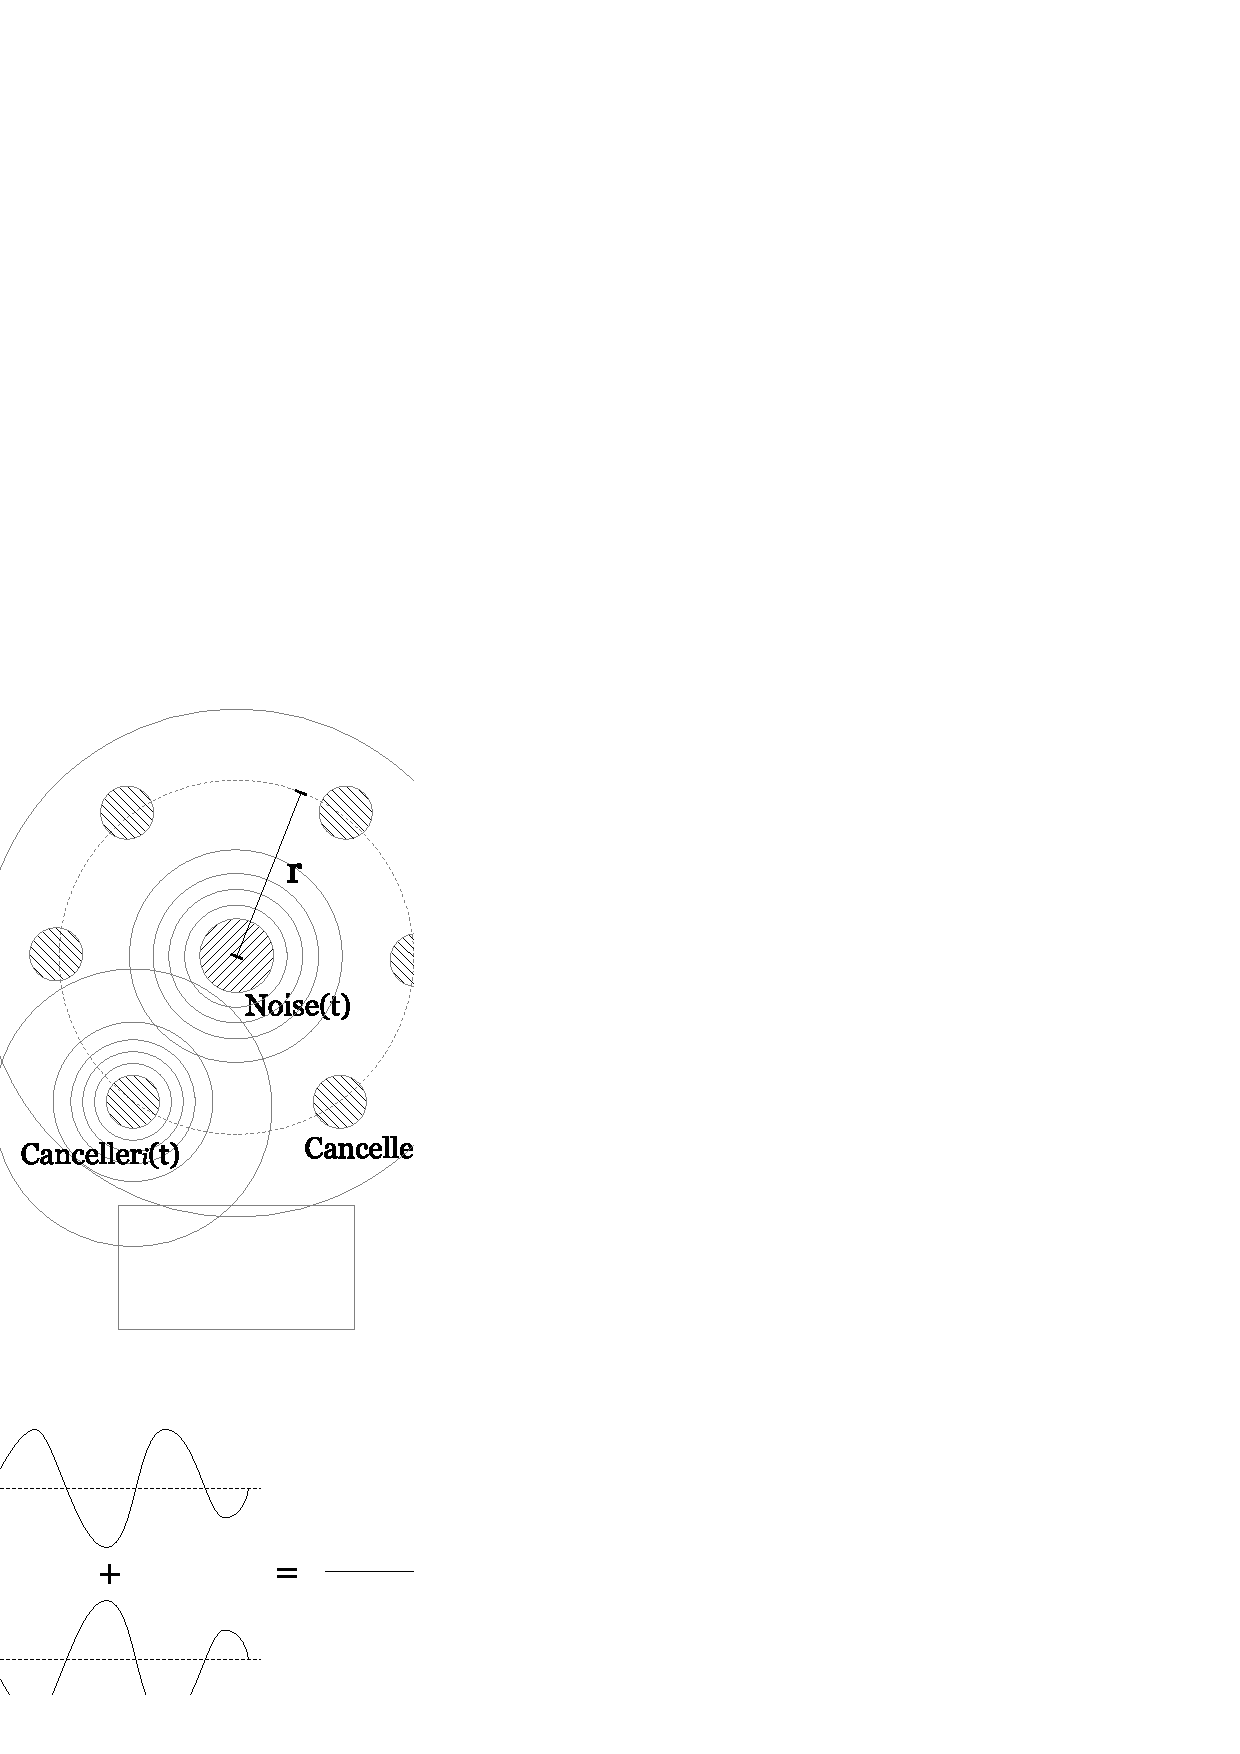
\includegraphics[bb=0mm 0mm 100.0mm 170.0mm, scale=0.35, type=pdf]{img/problem4.pdf}
\end{figure}
\end{column}
\end{columns}
\end{frame}


%%%%%%%%%%%%%%%%%%%%%%%%%%%%%%%%%%%%%%%%%%%%%%%%%%%%%%%%%%%%%%%%%%%%%%%%%%%%%%%%%%%%%%%%%%%%%%%%%%%%%%%%%%%%

\begin{frame}{問題5}{平行平板コンデンサのエッジ効果}
\begin{wideitemize}
\item 平行平板コンデンサの静電容量を求める
\begin{wideitemize2}
\item 実際のコンデンサの端では、電界は一様ではない \\
(エッジ効果)
\item $C=\dfrac{\epsilon_0 S}{d}$ よりも正確な容量
\item 電極は適当な大きさの長方形
\item エッジ効果を考慮した近似式と比較する
\end{wideitemize2}
\end{wideitemize}

\begin{figure}[htbp]
    \centering
    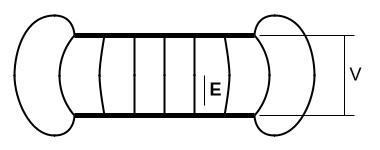
\includegraphics[width=200pt]{svg/capacitor.pdf}
\end{figure}
\end{frame}

%%%%%%%%%%%%%%%%%%%%%%%%%%%%%%%%%%%%%%%%%%%%%%%%%%%%%%%%%%%%%%%%%%%%%%%%%%%%%%%%%%%%%%%%%%%%%%%%%%%%%%%%%%%%

\begin{frame}{問題6}{飛行距離}
\begin{columns}[t]
\begin{column}{0.7\textwidth}
\begin{wideitemize}
	\item ペットボトルロケットを遠くまで飛ばしたい。最適な水の量、圧力、打ち上げ角度はいくつか?
	\begin{wideitemize2}
		\item 標準大気圧、25度で乾燥しており、無風
		\item 空気は粘性のない、比熱比1.4の理想気体
		\item ペットボトルは半径45mmで容積1.5Lの円柱で、耐圧0.6MPa
		\item ノズルは直径4mm、ロケットの先端は頂角60度の円錐
		\item 水を除いたロケット全体の重さは150g
		\item 必ずしも全ての条件を用いなくてよい。適当なモデルを考えること。
	\end{wideitemize2}
\end{wideitemize}

\end{column}
\begin{column}{0.3\textwidth}
\begin{figure}[htbp]
    \centering
    \includegraphics[bb=0mm 0mm 100.0mm 170.0mm, scale=0.35, type=pdf]{img/problem6.pdf}
	% http://atsites.jp/yoshitoharada/1150_Water-rocket1.jpg
\end{figure}
\end{column}
\end{columns}
\end{frame}

%%%%%%%%%%%%%%%%%%%%%%%%%%%%%%%%%%%%%%%%%%%%%%%%%%%%%%%%%%%%%%%%%%%%%%%%%%%%%%%%%%%%%%%%%%%%%%%%%%%%%%%%%%%%

\begin{frame}{問題7}{空間消音}
\begin{columns}[t]
\begin{column}{0.7\textwidth}
\begin{wideitemize}
	\item 救急車のサイレン音打消しをモデルとして、空間の消音をしたい。消音スピーカーから各々どのような波を出せばよいか
	\begin{wideitemize2}
		\item 幅(x軸)$1.6m$、長さ(y軸)$3.6m$、高さ(z軸)$2m$の大きさの直方体を考え、上面端に$(0, 0, 0)$座標を置く
		\item 960Hzで振幅1の正弦波を出すサイレンが$(0.8,1.8,0)$の位置にある
		\item 消音スピーカーは、高さ$1.6m$、壁面から$0.2m$離れた位置に4つ置く
		\item $(0.6, 2.0, 2.0)$、$(1.0, 2.0, 2.0)$、$(1.0, 2.4, 2.0)$、$(0.6, 2.4, 2.0)$を底面とし、高さが$0.4m$の立方体の空間でエネルギーを最小化する
		\item 標準大気圧で、乾燥しており、温度は20度とする。
	\end{wideitemize2}

\end{wideitemize}

\end{column}
\begin{column}{0.3\textwidth}
\begin{figure}[htbp]
    \centering
    \includegraphics[bb=0mm 0mm 100.0mm 170.0mm, scale=0.35, type=pdf]{img/problem7.pdf}
\end{figure}
\end{column}
\end{columns}
\end{frame}

%%%%%%%%%%%%%%%%%%%%%%%%%%%%%%%%%%%%%%%%%%%%%%%%%%%%%%%%%%%%%%%%%%%%%%%%%%%%%%%%%%%%%%%%%%%%%%%%%%%%%%%%%%%%

\begin{frame}{問題8}{流体力学}
\begin{columns}[t]
\begin{column}{0.7\textwidth}
\begin{wideitemize}
	\item 二次元翼として、ジューコフスキー翼の迎え角と揚力の関係を求めたい。
	\item だが、少し難しいので、平面板間を流れる二次元的な流体に図のように正方形の障害物を置いた際の流れの乱れを
	シミュレーションせよ。
	\begin{wideitemize2}
		\item 非圧縮性流体を仮定する。適当な流体(空気、あるいは水)を仮定せよ。
		\item 管の太さ、あるいは障害物の大きさを変えるとどのようなふるまいをするだろうか。
	\end{wideitemize2}
\end{wideitemize}

\end{column}
\begin{column}{0.3\textwidth}
\begin{figure}[htbp]
    \centering
    \includegraphics[bb=0mm 0mm 100.0mm 170.0mm, scale=0.35, type=pdf]{img/problem8.pdf}
\end{figure}
\end{column}
\end{columns}
\end{frame}

%%%%%%%%%%%%%%%%%%%%%%%%%%%%%%%%%%%%%%%%%%%%%%%%%%%%%%%%%%%%%%%%%%%%%%%%%%%%%%%%%%%%%%%%%%%%%%%%%%%%%%%%%%%%

\begin{frame}{問題9}{ベンゼン}
\begin{columns}[t]
\begin{column}{0.7\textwidth}
\begin{wideitemize}
	\item ベンゼン分子の電子軌道を計算することで、ベンゼンの炭素-炭素間結合が「1.5重結合」であることを確認したい。
	\begin{wideitemize2}
		\item いわゆる「ハートリー・フォック法」を用いること。
		\item 基底関数系に適当なガウス基底を用いること。
		\item ベンゼン分子中の各原子の位置は予め与えてよい。
		\item まずは、水素分子で試すこと。
	\end{wideitemize2}
\end{wideitemize}

\end{column}
\begin{column}{0.3\textwidth}
\begin{figure}[htbp]
    \centering
    \includegraphics[bb=0mm 0mm 100.0mm 170.0mm, scale=0.35, type=pdf]{img/problem9.pdf}
\end{figure}
\end{column}
\end{columns}
\end{frame}


%%%%%%%%%%%%%%%%%%%%%%%%%%%%%%%%%%%%%%%%%%%%%%%%%%%%%%%%%%%%%%%%%%%%%%%%%%%%%%%%%%%%%%%%%%%%%%%%%%%%%%%%%%%%

%
% 製作者のお願い:このスライドは、極めて的確に難易度を表現しながらも、
%         一方でひどく曖昧にも見えるため、問題選択者のプライドを傷つけません!
%         可能なら、消さないでください。
%

% http://clipart-animal.com/

\begin{frame}{問題の難易度や傾向}
\begin{columns}[t]
\begin{column}{0.5\textwidth}
\begin{wideitemize}
\item[1.] 熱伝導
\begin{figure}[htbp]
    \centering
    \includegraphics[bb=0 0 6.4 4.8, scale=0.07]{img/a01.jpg}
\end{figure}
\item[2.] 球充填
\begin{figure}[htbp]
    \centering
    \includegraphics[bb=0 0 6.4 4.8, scale=0.06]{img/a02.jpg}
\end{figure}
\item[3.] スイングバイ
\begin{figure}[htbp]
    \centering
    \includegraphics[bb=0 0 6.4 4.8, scale=0.08]{img/a03.jpg}
\end{figure}
\item[4.] トンネル効果
\begin{figure}[htbp]
    \centering
    \includegraphics[bb=0 0 6.4 4.8, scale=0.07]{img/a04.jpg}
\end{figure}
\item[5.] コンデンサ
\begin{figure}[htbp]
    \centering
    \includegraphics[bb=0 0 6.4 4.8, scale=0.08]{img/a05.jpg}
\end{figure}
\end{wideitemize}
\end{column}
\begin{column}{0.5\textwidth}
\begin{wideitemize}
\item[6.] PET-ロケット
\begin{figure}[htbp]
    \centering
    \includegraphics[bb=0 0 6.4 4.8, scale=0.07]{img/a06.jpg}
\end{figure}
\item[7.] 空間消音
\begin{figure}[htbp]
    \centering
    \includegraphics[bb=0 0 6.4 4.8, scale=0.08]{img/a07.jpg}
\end{figure}
\item[8a.] 流れの乱れ
\begin{figure}[htbp]
    \centering
    \includegraphics[bb=0 0 6.4 4.8, scale=0.09]{img/a08.jpg}
\end{figure}
\item[8b.] 翼
\begin{figure}[htbp]
    \centering
    \includegraphics[bb=0 0 6.4 4.8, scale=0.09]{img/a08_2.jpg}
\end{figure}
\item[9.] ベンゼン
\begin{figure}[htbp]
    \centering
    \includegraphics[bb=-300 0 6.4 4.8, scale=0.055]{img/a09.jpg}
\end{figure}
\end{wideitemize}
\end{column}
\end{columns}
\end{frame}

%%%%%%%%%%%%%%%%%%%%%%%%%%%%%%%%%%%%%%%%%%%%%%%%%%%%%%%%%%%%%%%%%%%%%%%%%%%%%%%%%%%%%%%%%%%%%%%%%%%%%%%%%%%%

\end{document}

